\documentclass{anvil-paper}
\usepackage{array}
\usepackage{float}
\newcommand{\Nm}{\mathrm{N\,m}}
\newcommand{\dd}{\,\mathrm{d}}
\title{Interface truncation and verified design gradients\\
in a nonlinear motor model}
\author{}
\date{October 2026}
\hypersetup{pdftitle={Interface truncation and verified design gradients in a nonlinear motor model},pdfsubject={Torque-ripple reproduction and discrete design-gradient verification}}

\begin{document}
\maketitle
\begin{abstract}
A motor optimization target can change with the numerical interface even
when average torque agrees closely. We reconstruct a published nonlinear
permanent-magnet motor with piecewise-linear finite elements and compare
conforming and harmonic rotor--stator coupling on identical meshes.
The conforming model reproduces loaded mean torque within 0.16\%, but its
torque standard deviation is 9.9--11.3\% above the saved reference.
Transmitting the reference's eight harmonic orders reduces that ripple
discrepancy to 1.3--1.7\% and the largest full-current waveform gap from
0.0272 to 0.0034\,N\,m. Cogging amplitude remains 12.9\% high, with reference
and geometry errors still unbounded. We then differentiate the converged
nonlinear model through mesh motion, excitation and torque evaluation.
Across 800 loaded finite-difference comparisons, 782 agree within
$2.8\times10^{-7}$ relatively; the largest error is $1.1\times10^{-5}$
on a small gradient component. The excitation rule can reverse the sign
of a design sensitivity. Recorded gradient evaluations cost 1.13--1.20
forward evaluations, compared with 7.2--9.5 for warm-started central
differences, under uncontrolled host load. These results establish an
objective-sensitive model comparison and discrete derivative verification;
optimization time to a common validated target remains to be measured.
\end{abstract}

\section{Introduction}
A small error in mean torque can conceal a large change in the quantity
being optimized. Reconstructing the initial motor of
\citet{wiesheu2024spline}, we find mean torque within 0.16\% of its saved
output while torque ripple differs by about 10--11\% under load.
Changing only the rotor--stator coupling to the published harmonic
truncation removes most of that gap. Thus a numerical modeling choice
changes the objective at a scale relevant to a torque-ripple study.

The same distinction applies to derivatives. An adjoint can produce many
design sensitivities without a field solve per parameter
\citep{scotzniovsky2024}, but it differentiates the chosen discrete model
and excitation policy. It does not establish that the objective is
resolved, or that following its gradients beats a cheaper design model.
These questions require separate checks of the field model, derivatives
and optimization outcome.

We report a four-mesh comparison of conforming and truncated harmonic
coupling, including two torque estimators and a harmonic-order ladder.
We also verify derivatives of mean torque and ripple with respect to
12 design parameters at initial and perturbed designs, and expose the
effect of holding current rather than current density fixed. The
contribution is a reproducible account of model and derivative errors in
this published benchmark. The numerical methods are established; the
results supply the evidence needed before comparing optimization costs.

\section{Related work}
\citet{wiesheu2024spline} combine spline-based rotor and stator shape
optimization with engineering parameters for a nonlinear permanent-magnet
synchronous motor. Their public implementation and saved outputs provide
the reproduction target here. Their related study compares parameter and
shape optimization with isogeometric analysis
\citep{wiesheu2025combined}. We inherit the initial geometry, material
table and excitation conventions; we replace the field discretization and compare two
rotor--stator couplings. The resulting comparison is between numerical
models, rather than a comparison with a measured physical motor.

Differentiable motor design is established prior work.
\citet{scotzniovsky2024} combine geometric deformation, mesh motion and
electromagnetic analysis with adjoint-based derivatives. The existence of
a differentiable implementation is therefore insufficient as a novelty
claim. A useful comparison must establish what designs can be reached,
how accurately they are evaluated and how much computation is required.

Harmonic rotor--stator coupling is also established.
\citet{bontinck2018isogeometric} use separate isogeometric subdomains and
harmonic interface constraints; their exact circular geometry avoids
polygonal air-gap error. \citet{egger2022torque} derive torque from the
energy of a harmonic mortar formulation and examine its numerical
accuracy for ripple evaluation. We compare that coupling torque with the
gap-averaged stress expression of \citet{arkkio1987}. These works motivate
checking interface order, field resolution and torque evaluation together,
rather than treating small mean-torque error as sufficient validation.
Mesh selection for torque computation is itself an established concern
\citep{arkkio2012proper}.

\citet{ion2018robust} compare deterministic gradient-based optimization
with stochastic search for electric devices, including a permanent-magnet
motor, using geometry parametrizations that avoid remeshing. Therefore,
a gradient-versus-stochastic comparison or a differentiable motor solver
alone would not establish a new optimization result. Our eventual cost
comparison must also include competitive inexpensive models and evaluate
all candidates against a common refined target.

Inexpensive alternatives also need substantive treatment.
\citet{kemmetmueller2015} use nonlinear magnetic equivalent circuits for
torque control, including saturation and nonsinusoidal behavior. Their
control problem differs from shape optimization, but it demonstrates why
saturation alone does not establish the need for a full-field model.
\citet{roomi2022} develop a waveform-targeting surrogate for electrical
machine design, while \citet{wen2023} adapt reduced models along a
shape-optimization trajectory in fluid examples. These approaches motivate
waveform-aware and adaptive baselines. Their published performance is not
transferred to the motor studied here.

\section{Motor model and reconstruction}
\subsection{Geometry and operating states}
The full machine has six poles and 36 stator slots. We model a
$60^\circ$ sector, occupying $60^\circ\leq\theta\leq120^\circ$ at zero
rotation, with antiperiodic conditions on the radial boundaries. The rotor
inner and outer radii are 16 and 44\,mm; the stator inner and outer radii
are 45 and 67.5\,mm. Axial length is $L=0.1$\,m. The 1\,mm air gap is
split at the coupling radius $r_c=44.5$\,mm. Figure~\ref{fig:geometry}
shows the material-tagged reconstruction.

\begin{figure}[htbp]
\centering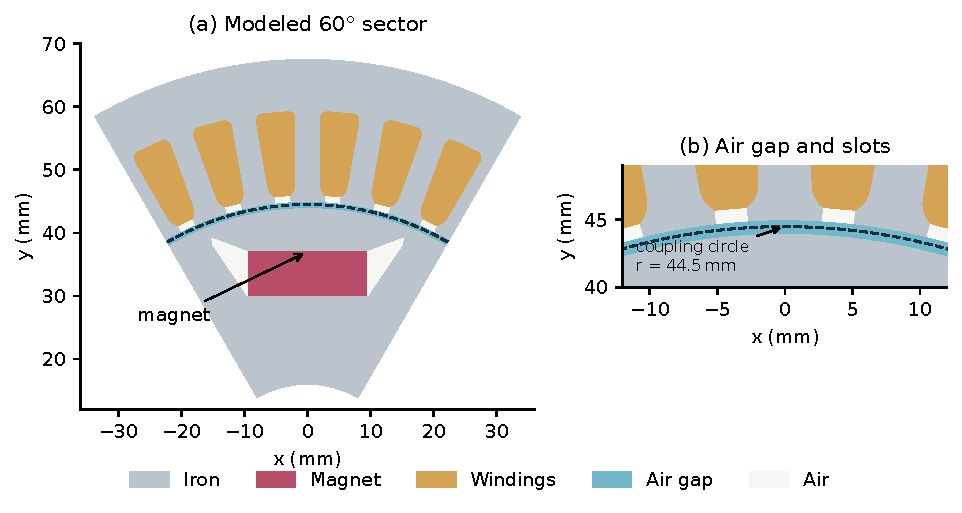
\includegraphics[width=\linewidth]{figures/geometry.pdf}
\caption{Initial-design geometry rendered directly from the committed
coarsest mesh. The dashed line is the rotor--stator coupling circle. The
right panel enlarges the gap and slot openings. Material boundaries are
shown without the element edges; the geometry is not an optimized result.}
\label{fig:geometry}
\end{figure}

The reconstruction uses the initial NURBS exports in the public snapshot.
Their control points are stored with weights already multiplied in, and
patch orientation must be accounted for when integrating areas. Two thin
rotor patches described as air slits in source comments receive iron under
the reference's material assignment; we follow that assignment. The
mesh generator preserves the winding groups separately, since their two
characteristic areas are approximately 36.29 and 31.22\,mm$^2$.

At mechanical angle $\beta$, phase currents are
\begin{equation}
 I_q(\beta)=a I_*\sin(\phi_0+3\beta+\delta_q),\qquad
 (\delta_U,\delta_V,\delta_W)=(0,-2\pi/3,2\pi/3),
 \label{eq:current}
\end{equation}
where $a\in\{0,0.5,1\}$, $I_*=9.677657374$\,A, and the electrical phase
offset $\phi_0=0$ for the initial design. Angles in
Eq.~\eqref{eq:current} are in radians. Each winding group carries current
density $J_g=12s_g I_q/|\Omega_g|$, with its own area and prescribed sign
$s_g\in\{-1,1\}$. Using a common area would change the current density
between groups by about 16\%. We compare 20 distinct mechanical angles,
$0^\circ,1^\circ,\ldots,19^\circ$, excluding the duplicated endpoint in
the source CSV. The reference's optimization grid contains the ten even
angles; both grids are retained in the artifacts.

\subsection{Nonlinear field equation}
The two-dimensional magnetic vector potential $A=A_z$ determines the
flux density $\mathbf B=(\partial_y A,-\partial_x A)$. Iron is described
by an isotropic reluctivity $\nu(|\mathbf B|^2)$, where reluctivity is
the inverse of permeability. For a test function $v$ that satisfies the
homogeneous constraints, the weak equation is
\begin{equation}
 \int_\Omega \nu(|\nabla A|^2)\nabla A\cdot\nabla v\dd\Omega
 =\int_\Omega J_z v\dd\Omega
  +\int_{\Omega_m}\mathbf M\cdot(\partial_y v,-\partial_x v)\dd\Omega.
 \label{eq:weak}
\end{equation}
Here $\mathbf M$ denotes the permanent-magnet source in
$\mathbf H=\nu\mathbf B-\mathbf M$. In the magnet,
$\mu_r=1.05$ and $B_r=1.4$\,T, so its source magnitude is
$H_c=B_r/(\mu_0\mu_r)$, not $B_r/\mu_0$. Its direction is $\pi/2$
in the rotor frame and rotates with the rotor. Air and windings have
$\mu_r=1$. The inner and outer circular boundaries have $A=0$.

We use continuous piecewise-linear triangles. With nodal vector $u$,
element gradients $g_i=\nabla\varphi_i$, $G=\nabla A$ and $s=G\cdot G$,
the residual derivative on one element is
\begin{equation}
 K^e_{ij}=|\Omega_e|\left[\nu(s)g_i\cdot g_j
       +2\nu'(s)(g_i\cdot G)(g_j\cdot G)\right].
 \label{eq:tangent}
\end{equation}
The second term is required when the material changes with field strength.
Newton steps use this consistent tangent, with damping and a stopping
reference independent of the initial guess. Constant potential offsets,
where allowed by the boundary conditions, do not change that reference.
The solver reports whether it stopped at the requested tolerance or an
estimated floating-point floor. All 500 baseline and sensitivity solves, and all 1,140
additional harmonic-coupling solves, stopped at the requested tolerance.

The iron law uses 47 tabulated M27 $B$--$H$ points from 0 to 2.30\,T.
Monotonicity is imposed on $H(B)$, not on $\nu(B^2)=H(B)/B$.
The tabulated $H/B$ is non-monotone up to about 0.75\,T.
The two material tangent eigenvalues must satisfy
\begin{equation}
 \nu>0,\qquad \nu+2s\nu'=\frac{\dd H}{\dd B}>0.
\end{equation}
The GEODE and reference interpolants agree to round-off between 0.05 and
2.25\,T. GEODE uses an odd cubic near zero and a continuous slope into the
vacuum-slope tail above 2.30\,T. The reference uses a low-field clamp and
a different last-knot slope. The maximum relative difference in
reluctivity near zero is 6.66\%; the last segment differs in $H$ by at
most $2.17\times10^{-4}$ relatively. We test the torque effect of the
low-field difference in Section~\ref{sec:sensitivity}.

\subsection{Rotation and torque}
At the modeled angles, the two circular traces have matching nodes after
rotation. The sliding interface identifies their potentials, including
the antiperiodic sign on sector wrap-around. Writing the full nodal vector
as $u=P\hat u+u_D$, the reduced residual and tangent are
$\hat R=P^T R(P\hat u+u_D)$ and $\hat K=P^T K P$.
The rotor geometry and magnet source rotate together; currents use the
same mechanical angle in Eq.~\eqref{eq:current}.

We average Maxwell stress over the air gap using the Arkkio expression
\citep{arkkio1987}
\begin{equation}
 T(\beta)=\frac{L}{\mu_0(r_2-r_1)}
  \int_{\Omega_{\rm gap}}r B_r B_\theta\dd\Omega,
 \qquad(r_1,r_2)=(44,45)\ {\rm mm}.
 \label{eq:torque}
\end{equation}
Positive torque acts counter-clockwise on the rotor. All torques in this
paper include axial length and refer to the modeled sector. We apply no
factor of six when comparing with the saved reference arrays, despite a
per-length label appearing in the reference evaluation plots.

The alternative harmonic model imposes
\begin{equation}
 \int_{\Gamma_c}(A_s-A_r)e_n\dd\Gamma=0,\qquad
 e_n\in\{\sin(n\theta),\cos(n\theta)\},\quad n=3,9,\ldots,45.
\end{equation}
The 16 constraints match the reference's eight orders. Rotor and stator
retain distinct trace unknowns. With constraint matrix $C$, Lagrange
multipliers $\eta$ and reduced potential $\hat u$, Newton's method uses
the saddle tangent
\begin{equation}
 \begin{bmatrix}K&C\\ C^T&0\end{bmatrix}.
\end{equation}
The trace moments use the exact Fourier integrals of the piecewise-linear
hats. Rotation enters their centers; the constrained energy derivative gives
\begin{equation}
 T_c=-L\eta^T\frac{\partial(C^T\hat u)}{\partial\beta},
 \label{eq:couplingtorque}
\end{equation}
with the state held fixed in the partial derivative, consistent with
\citet{egger2022torque}. Forward comparisons use Arkkio for both GEODE
couplings to isolate the interface change; coupling torque is a separate
check. The derivative study uses coupling torque for the harmonic model
and Arkkio for the conforming model. The two objectives and their gradients
are consequently comparisons of those specified model--estimator pairs.

The main harmonic runs retain antiperiodic trace-end pairing. An additional
set frees those ends, matching the reference's treatment. Increasing the
transmitted orders to every mode below the trace Nyquist limit reproduces
the conforming Arkkio torques within $4.1\times10^{-9}$\,N\,m on L0 and
$1.3\times10^{-9}$\,N\,m on L1. This checks the interface implementation
without fitting any parameter to the saved torque.

\section{Verification and experiment design}
The implementation is checked before the motor comparison. With constant
material laws it agrees with the linear assembly to approximately
$2\times10^{-14}$ in potential. Central differences of the nonlinear
residual agree with the tangent action to below $10^{-9}$ at favorable
step sizes on the synthetic material tests. A manufactured solution gives
fitted spatial rates 1.002 in the $H^1$ seminorm and 2.007 in $L^2$.
For a saturated iron annulus carrying enclosed current $I$, the independent
radial field relation is $H(r)=I/(2\pi r)$, followed by inversion of the
material law. The M27 test reaches a mid-annulus relative field error of
$3.76\times10^{-4}$ on its finest mesh. These are verification results
for the forward model; they do not verify motor shape derivatives.

Sector tests compare the constrained solution with a full-machine solve,
check the reduced tangent by finite differences, and exercise positive,
negative and wrapped rotation steps. Clockwise and counter-clockwise
triangle orderings give equivalent magnet sources and fields. The motor
regression also detects changes in magnet strength, magnet direction,
phase ordering and rotation direction. Detailed logs accompany the code.

The motor study uses four meshes, L0--L3, with 3,153, 9,937, 36,083 and
139,268 nodes. The $60^\circ$ coupling arc has $120\,2^\ell$ segments at level
$\ell$, so integer-degree rotation is represented at every level.
Each level contains 60 baseline solves: three current levels and 20
angles. A solution at one angle initializes the next angle at the same
current. We report the mean and population standard deviation,
\begin{equation}
 \bar T=\frac1N\sum_{k=1}^N T_k,\qquad
 \sigma_T=\left[\frac1N\sum_{k=1}^N(T_k-\bar T)^2\right]^{1/2},
 \quad N=20.
\end{equation}
The standard deviation is the ripple metric used for the comparison.
At zero current it measures cogging, the torque variation caused by the
permanent magnets and slots without applied phase current.

For a scalar statistic $q$, the estimated L3 refinement interval is
\begin{equation}
 q_3\ \pm\ e_q,\qquad
 e_q=\max\{|q_2-q_1|,|q_3-q_2|\}.
 \label{eq:band}
\end{equation}
We use the same construction pointwise for waveforms. This interval is a
refinement diagnostic, not a proven error bound or a statistical confidence
interval. It does not cover reference-model error or angular quadrature
error. The loaded means change direction between the last two increments,
so a last-increment estimate alone would be particularly weak.

\section{Forward reproduction results}
\subsection{Coupling changes the ripple objective}
Table~\ref{tab:torque} compares the same geometry, material and excitation
with two interface models. The conforming L3 means are 0.15\% and 0.16\%
low at half and full current. Harmonic coupling reduces the mean deviations
to $-0.002\%$ and $+0.051\%$, with both reference means inside the estimated
refinement intervals. The loaded ripple deviations fall from $+9.9\%$
and $+11.3\%$ to $+1.7\%$ and $+1.3\%$.

\begin{table}[htbp]\centering\small
\caption{L3 population standard deviation and mean torque, in N\,m per
sector, on the 20-angle grid. The last column gives ripple deviation from the
saved reference. Relative zero-current mean error is not used.}
\label{tab:torque}
\begin{tabular}{llrrr}\toprule
Current fraction & Model & Mean & Std & Std deviation\\\midrule
0 & Reference & 0.00010 & 0.01071 & n/a \\
0 & Conforming & 0.00001 & 0.00760 & -29.1\% \\
0 & Harmonic & -0.00000 & 0.01209 & +12.9\% \\
0.5 & Reference & 0.66208 & 0.03895 & n/a \\
0.5 & Conforming & 0.66106 & 0.04279 & +9.9\% \\
0.5 & Harmonic & 0.66206 & 0.03961 & +1.7\% \\
1 & Reference & 1.44248 & 0.07935 & n/a \\
1 & Conforming & 1.44023 & 0.08829 & +11.3\% \\
1 & Harmonic & 1.44322 & 0.08036 & +1.3\% \\
\bottomrule\end{tabular}

\end{table}

Figure~\ref{fig:waveforms} shows the improvement angle by angle. The largest
full-current difference falls from 0.0272 to 0.0034\,N\,m. The harmonic
full-current ripple interval contains the saved reference; the half-current
value lies approximately $5\times10^{-5}$\,N\,m below its interval.
Mean agreement is therefore insufficient to characterize waveform accuracy.

\begin{figure}[htbp]\centering
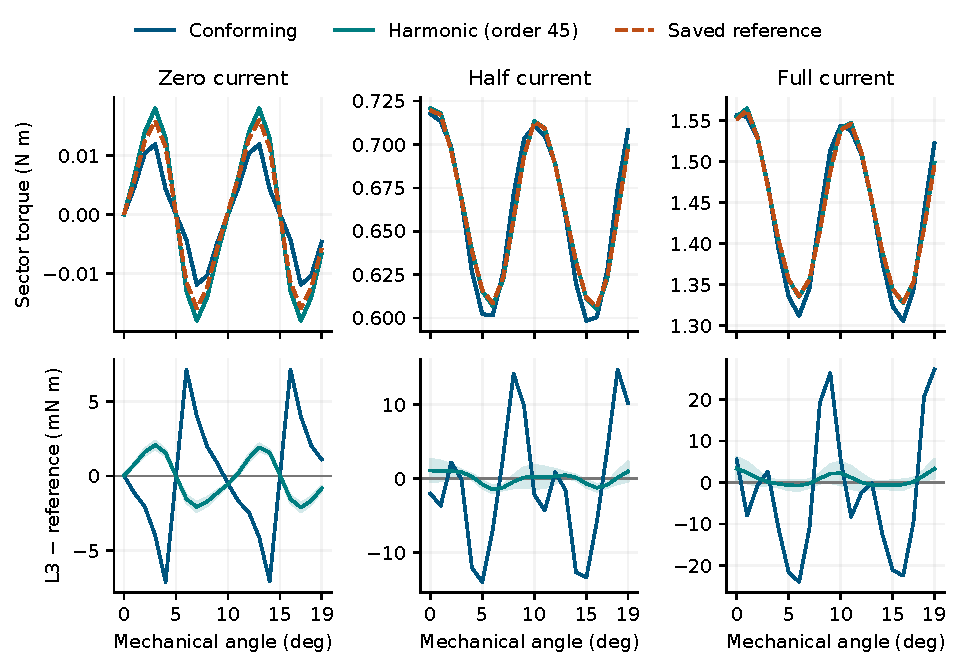
\includegraphics[width=\linewidth]{figures/coupling-waveforms.pdf}
\caption{Top: L3 torque for conforming and order-45 harmonic coupling,
compared with the saved reference. Bottom: each GEODE waveform minus the
reference; shading is the harmonic model's pointwise estimated refinement
interval from Eq.~\eqref{eq:band}. Residual panels have independent scales.
All GEODE curves use Arkkio torque, so the paired difference changes the
coupling while holding the estimator fixed.}
\label{fig:waveforms}\end{figure}

The zero-current result is less resolved. Harmonic coupling changes the
cogging standard deviation from 29.1\% below to 12.9\% above the reference.
Its waveform is close to a 1.13-fold scaling of the saved waveform, but the
reference lies outside the estimated ripple interval. We retain this
amplitude mismatch rather than interpreting improved waveform shape as a
complete reproduction.

\subsection{Spatial resolution and transmitted order}
Spatial refinement at fixed order and order refinement on a fixed mesh
answer different questions (Fig.~\ref{fig:convergence}). At L3, order 45
and the conforming model differ in ripple by about 59\% at zero current
and 7--9\% under load, relative to the conforming values. At L1 and L2,
order 189 approaches the conforming torque to within $1.1\times10^{-4}$\,N\,m.
A spatially refined order-45 solution thus remains a solution of a
truncated interface model. Matching that truncation improves reproduction
of the published calculation; it does not establish which model better
represents the physical motor.

\begin{figure}[htbp]\centering
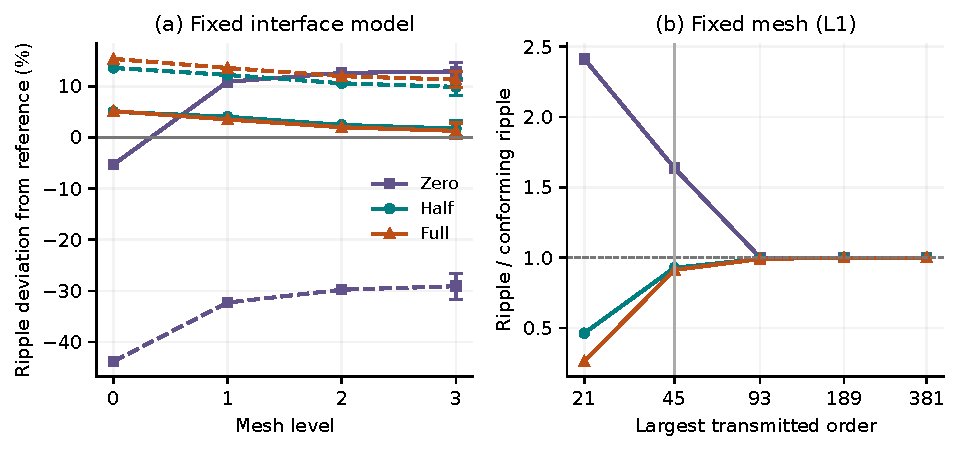
\includegraphics[width=\linewidth]{figures/coupling-convergence.pdf}
\caption{Left: ripple deviation from the reference under spatial
refinement, with solid lines for harmonic order 45 and dashed lines for
conforming coupling; L3 bars use Eq.~\eqref{eq:band}. Right: order
refinement on L1, normalized by the conforming ripple at that same level.
The reference uses order 45. Colors identify current, not coupling.}
\label{fig:convergence}\end{figure}

Two additional controls narrow the explanation. At L3, coupling torque
and the inner- and outer-half Arkkio estimates are each within
$9\times10^{-5}$\,N\,m of full-band Arkkio in the order-45 solution.
Freeing the coupling-arc ends changes torque by less than
$5.4\times10^{-5}$\,N\,m. These effects are too small to explain the remaining
cogging gap at the tested resolution.

\subsection{Sensitivity and unresolved causes}\label{sec:sensitivity}
The controlled changes in Table~\ref{tab:sensitivity} are too small to
explain the observed waveform gap at the tested settings. The near-zero
material difference has particularly little effect on torque despite its
6.66\% local reluctivity difference. This is a measured sensitivity of
the initial design and does not establish insensitivity after optimization.

\begin{table}[htbp]\centering\small
\caption{Maximum absolute torque change relative to the baseline at the
same mesh level. Entries summarize the recorded angle/current subsets.}
\label{tab:sensitivity}
\begin{tabular}{p{.48\linewidth}ll}\toprule
Change & Levels & Max. $|\Delta T|$ (N\,m)\\\midrule
Reference low-field interpolation and clamp & L2, L3 & $2.1\times10^{-6}$\\
Relative Newton tolerance $10^{-12}$ vs $10^{-8}$ & L2; L3 full current & $7.3\times10^{-8}$\\
Exact winding areas vs mesh areas & L2 & $3.9\times10^{-4}$\\
Inner or outer half of the Arkkio band & L3 & $7.3\times10^{-5}$\\
\bottomrule\end{tabular}
\end{table}

Single-circle Maxwell-stress estimates are more sensitive to the
piecewise-constant field than the gap average. The paired coupling-torque
and half-band checks above provide stronger support for the estimator
than selecting a favorable integration radius.

Filtering a solved conforming field is not equivalent to imposing a
truncated interface during the field solve. For completeness, the earlier
order-45 post-processing diagnostic changed the cogging standard deviation
from about 0.0075 to 0.0184\,N\,m, the half-current value from 0.04280 to
0.04460, and the full-current value from 0.08832 to 0.08775. The zero-current
values at cuts 9, 21, 45, 93 and 189 were 0.0077, 0.0300, 0.0184, 0.0077
and 0.0075. That non-monotone diagnostic neither supports nor excludes the
coupling explanation. The paired field solves, which reduce both loaded
discrepancies, supply the evidence for it.

The remaining cogging difference has unbounded contributions from the
reference's degree-two isogeometric discretization with $3\times3$
subdivisions per patch and from GEODE's straight-sided approximation of
curved material boundaries. The reference has not been rerun at finer
resolution. Torque-method differences have been measured within GEODE,
but a cross-code comparison on the same converged fields is unavailable.
The iron-law check covers the low-field difference only: the final tabular
segment and the extrapolated high-field regime have not been varied in a
paired torque experiment, although local bridge fields exceed the table.
These limitations preclude assigning the residual cogging error to a
single cause.

\section{Design-gradient verification}\label{sec:gradients}
\subsection{Differentiated model and excitation policy}
For a design vector $p$, the converged state $z$ contains the reduced
potential and, for harmonic coupling, its multipliers. Writing the full
constrained residual as $R(z,p)=0$, the discrete adjoint is
\begin{equation}
 R_z^T\psi=F_z^T,\qquad
 \frac{\dd F}{\dd p}=F_p-\psi^T R_p.
 \label{eq:adjoint}
\end{equation}
We differentiate mesh coordinates, element terms, magnet sources, current
loads, harmonic constraints and the torque functional. The explicit
coordinate derivative of Arkkio is included for conforming coupling.
Fixed-topology mesh motion $X(p)$ supplies the chain rule
$\dd F/\dd p_k=\langle\dd F/\dd X,\partial X/\partial p_k\rangle$
for geometric parameters, with direct terms added where needed.

The 12 parameters comprise nine geometric lengths (MAG, MH, MW,
SW1--SW4, SD1 and Sr1), axial length, operating angle and radial scale.
The two designs are the initial parameters and an interior point halfway
toward the saved optimized scalar parameters
(Appendix~\ref{sec:parameters}). This verifies a local scalar
parametrization. The reference's optimized geometry also uses grouped
surface-control displacements; reproducing its 12 scalar values alone
does not reproduce that geometry. The present gradient comparison does
not include derivatives of those additional groups or a new optimized
motor.

The primary current rule fixes peak current, so
$J_g=12s_g I_q/|\Omega_g(X)|$ changes when a slot changes area.
For comparison we implement the reference optimizer's rule, denoted
\emph{fixed group-1 density}: $I_*\propto |\Omega_1(X)|s$, where $s$ is
radial scale, with the proportionality constant fixed at the initial
design. The unscaled geometry is evaluated and torque is multiplied by
$s^2$, following the reference. Both rules agree at the initial geometry
but have different derivatives. At L1 with harmonic coupling and full
current, the mean-torque derivative with respect to SW1 is
$+1.68$\,N\,m/m under fixed current and $-220.85$\,N\,m/m under fixed
group-1 density (Fig.~\ref{fig:gradients}). SW1 is the stator-tooth-width
parameter. The sign change comes from the additional winding-area/current
term, not an adjoint discrepancy. A future optimization comparison must
hold this policy fixed across methods.

\subsection{Finite differences and Taylor remainders}
The derivative objectives are mean torque and population standard
deviation on the ten even mechanical angles, matching the reference's
optimization grid. Central differences move the same mesh at $p\pm h e_k$;
step sweeps separate truncation from floating-point and nonlinear-solve
error. We also check the first-order remainder
$|F(p+h e_k)-F(p)-h\,\dd F/\dd p_k|$ for quadratic decay.

Across initial and perturbed designs, both couplings, L0--L2 and the
recorded loaded current/rule subsets, there are 800 objective--parameter
comparisons. Of these, 782 have a best-step relative error at most
$2.8\times10^{-7}$; the maximum is $1.07\times10^{-5}$ for a small Sr1
ripple derivative. This is a best-step verification statistic, not the
accuracy of a single finite-difference step chosen in advance.
Figure~\ref{fig:gradients} includes all 800 cases as well as one explicit
Taylor sweep. The artifact retains each step, rejected displacement and
relative error. Not every combination is run on every mesh; the count
refers to the recorded cases, not a full factorial study.

\begin{figure}[htbp]\centering
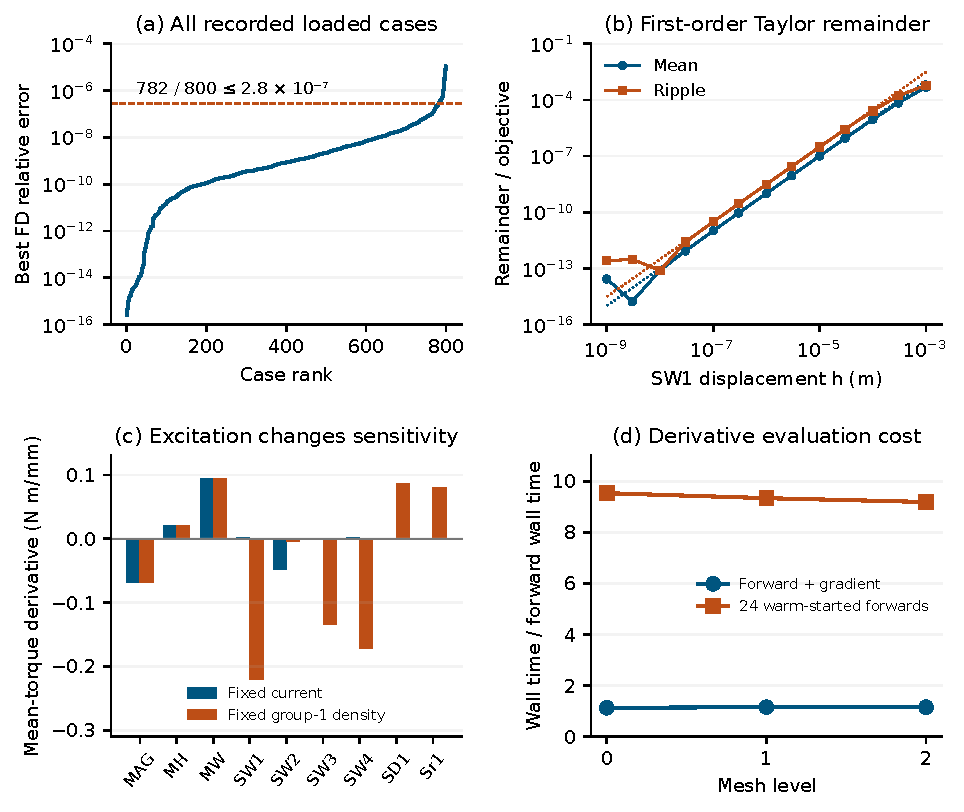
\includegraphics[width=\linewidth]{figures/design-gradients.pdf}
\caption{Discrete gradient evidence. (a) All 800 loaded best-step
finite-difference errors, sorted; each point is one recorded
objective--parameter case. (b) SW1 Taylor remainders at L1, initial design,
full current, harmonic coupling, fixed current; the guide is anchored at
$h=10^{-5}$\,m. (c) Mean-torque sensitivities for the nine geometric
parameters under two current rules at that same state. (d) Recorded cost
ratios for harmonic coupling at tolerance $10^{-14}$; gradients include
the forward evaluation. L0/L1 are medians of three runs, L2 a single run.
These timing data were collected under uncontrolled host load.}
\label{fig:gradients}\end{figure}

Taylor sweeps show quadratic regions, with smaller gradients reaching
round-off sooner. An anchored-window diagnostic fails for two loaded SW1
ripple cases because the remainder changes sign near the anchor; their
widest quadratic windows span two decades. The nearly cancelling
zero-current mean is a weaker check: its best relative errors reach
$7.0\times10^{-4}$. Cogging standard-deviation errors are at most
$8.9\times10^{-7}$. Thus the loaded agreement does not describe every
zero-current derivative.

Discrete derivative accuracy also does not imply mesh convergence. In the
harmonic model, SW3 mean-torque sensitivities change sign between coarse
levels and converge approximately linearly; ripple gradients converge
more slowly than most mean gradients. Fresh-remesh finite differences for
MW, SW1 and SW2 show decreasing discrepancies from moved-mesh derivatives,
but small remeshing steps are dominated by changes in connectivity. For
example, the fitted full-current MW mean derivative gap falls from about
$5.4\times10^{-3}$ relatively at L0 to below the remesh-scatter resolution
at L2; the fitted $2.6\times10^{-6}$ value is not a resolved accuracy bound.
These checks support the discrete chain rule while leaving refinement of
candidate designs necessary.

\subsection{Recorded derivative cost}
The recorded timings use an Apple M3 Ultra with 28 cores, default solver
threading, and concurrent host load averaging 14--24. The effective thread
count was not pinned. A forward evaluation covers ten angles, starts from
zero, and warm-starts successive angles. The full gradient includes that
forward, ten torque adjoints, mesh derivatives and contractions for all
12 parameters and both aggregate objectives. Both aggregates reuse the
per-angle torque derivatives. Central differences use 24 forward sweeps,
each warm-started from the base states.

Across L0--L2, both couplings and tolerances $10^{-8}$ and $10^{-14}$, the
full gradient costs 1.13--1.20 forwards, whereas central differences cost
7.2--9.5. Table~\ref{tab:cost} gives the harmonic tight-tolerance subset.
Shape-map setup is recorded separately and must be included in a complete
optimization budget. The timing advantage concerns derivative evaluation
on one loaded host. It provides no measurement of optimizer iterations,
surrogate calibration cost or time to a validated target.

\begin{table}[htbp]\centering\small
\caption{Recorded harmonic-model cost at relative tolerance $10^{-14}$,
initial design and full current. Times are seconds for ten-angle sweeps;
setup is a one-time shape-map cost.}
\label{tab:cost}\begin{tabular}{lrrrr}\toprule
Mesh & Forward & Forward + gradient & Central FD & Setup\\\midrule
L0 & 0.664 & 0.748 & 6.333 & 0.011 \\
L1 & 3.174 & 3.658 & 29.637 & 0.041 \\
L2 & 12.702 & 14.644 & 116.687 & 0.222 \\
\bottomrule\end{tabular}

\end{table}

\section{Discussion and limitations}
The controlled interface change explains most of the loaded ripple gap
while preserving mean-torque agreement. The order ladder shows why this
matters for optimization: interface truncation changes the objective even
as spatial error decreases. A gradient of that objective can be
numerically correct and inexpensive while pointing toward a design whose
improvement does not survive a change in the model.

The model is two-dimensional and magnetostatic. It does not evaluate
thermal behavior, demagnetization, fatigue, end effects, losses or a
complete efficiency map. The comparison uses published computational
artifacts, with no new measurements on a physical motor. The strongest
forward comparison concerns the initial design; local derivative tests
at a second design do not validate an optimization trajectory. Denser
and shifted angular grids, tighter spatial resolution and additional
current levels remain necessary for candidate validation.

A useful next comparison fixes the outer envelope, axial length, excitation
policy and geometric constraints, then measures time to the same refined
ripple target. It should separately compare optimization methods in a
common space and additional shape freedom under common constraints.
The reference already combines scalar and surface controls, so their
combination alone is not a new contribution. Costs must include mesh
updates, solves, gradients, line searches and calibration, with equivalent
reuse allowed to each method and failed targets reported explicitly.

A cheap waveform or reduced physical model is an essential baseline.
The linear slotless screening control in Appendix~\ref{sec:slotless}
admits a three-coefficient angular fit at one geometry. That does not
establish generalization across shapes, but it cautions against inferring
an optimization advantage from parameter count or adjoint cost alone.

\section{Conclusion}
On identical meshes of a published nonlinear motor, matching the
reference's harmonic interface reduces the loaded ripple discrepancy
from 9.9--11.3\% to 1.3--1.7\%. The remaining 12.9\% cogging-amplitude
difference is unresolved. Design gradients pass finite-difference and
Taylor checks at two parameter points, while a change in excitation
policy can reverse a sensitivity. The results establish model-specific
ripple and derivative evidence. Demonstrating a practical speedup requires
the next experiment: optimization against strong inexpensive baselines
at a common independently refined target.

\section*{Code and data availability}
The evidence used here is fixed at GEODE commit
\href{https://github.com/rjwalters/geode-fem/tree/910593bad6f64f9f01671c2632b57034e72b9c61}{\texttt{910593ba}}.
The repository contains the
\href{https://github.com/rjwalters/geode-fem/tree/910593bad6f64f9f01671c2632b57034e72b9c61/benchmarks/motor_reference/forward_harmonic}{raw motor runs and analysis},
\href{https://github.com/rjwalters/geode-fem/tree/910593bad6f64f9f01671c2632b57034e72b9c61/benchmarks/motor_reference/geometry}{geometry and mesh-generation scripts},
\href{https://github.com/rjwalters/geode-fem/tree/910593bad6f64f9f01671c2632b57034e72b9c61/benchmarks/motor_shape_gradient/design}{design-gradient sweeps and timing records},
and \href{https://github.com/rjwalters/geode-fem/tree/910593bad6f64f9f01671c2632b57034e72b9c61/benchmarks/motor_nonlinear_m1}{solver verification logs}.
Reference data are extracted from the authors'
\href{https://github.com/MichaelWiesheu/ICEMsnapshot/tree/b145aaf4ab1a6424828bc941eaf172f48fa0d458}{ICEM snapshot at \texttt{b145aaf4}},
a later repository revision rather than a claim to the original conference
release. Source hashes, extraction checks and the upstream GPL-3.0-or-later license
are retained. The paper package includes a manifest, copied figure inputs
and a regeneration script; it does not require rerunning FEM to rebuild
the figures. Recomputing the physical study requires the separately
documented mesh and solver commands.

\appendix
\section{Linear slotless screening control}\label{sec:slotless}
The stored slotless model has 24 distinct angles. Fitting
$T(\phi)=c_0+c_1\cos\phi+c_2\sin\phi$, with electrical angle $\phi=p\theta_r$, mechanical rotor angle $\theta_r$
and pole-pair count $p$, on alternate angles and
evaluating on the other twelve gives normalized held-out RMSE
$3.08\times10^{-10}$ and maximum error $6.83\times10^{-10}$, using the
recorded analytic-amplitude normalization. This is a locked-rotor angle sweep,
not synchronous operating ripple. For a fixed linear field operator and
sinusoidal sources, the field lies in a small basis of source responses;
a quadratic torque functional can contain only the corresponding finite
set of harmonics. The particular model needs just the three fitted
coefficients. This is an angular interpolation test at one geometry,
not a shape-gradient test or evidence of generalization across designs.

\section{Design points for derivative checks}\label{sec:parameters}
Table~\ref{tab:parameters} identifies the coordinates used in the scalar
derivative study. Values are rounded for display; the accompanying records
retain full precision. The operating angle is stored in degrees and
converted to radians in the current equation. These coordinates describe
the scalar design space; the saved reference optimum additionally contains
surface-control offsets.
\begin{table}[H]\centering\small
\caption{Initial and interior perturbed design points for the derivative
checks. Lengths refer to the unscaled geometry.}\label{tab:parameters}
\begin{tabular}{lp{.39\linewidth}lrr}\toprule
Parameter & Meaning & Unit & Initial & Perturbed\\\midrule
MAG & Pole-axis iron depth above magnet & mm & 7.0000 & 6.5506 \\
MH & Radial magnet height & mm & 7.0000 & 4.8722 \\
MW & Magnet width & mm & 19.0000 & 19.8670 \\
SW1 & Stator tooth width & mm & 4.0000 & 4.0309 \\
SW2 & Slot-opening width & mm & 2.3000 & 1.6500 \\
SW3 & Slot-opening depth & mm & 1.0000 & 0.7502 \\
SW4 & Back-iron depth on slot axis & mm & 8.2500 & 6.8418 \\
SD1 & Stator outer diameter & mm & 135.0000 & 132.6466 \\
Sr1 & Slot-bottom fillet radius & mm & 1.0000 & 1.4999 \\
LENGTH & Axial length & mm & 100.0000 & 90.0003 \\
$\phi_0$ & Electrical current offset & $^\circ$ & 0.0000 & -5.8231 \\
ScaleR & Radial similarity scale & 1 & 1.0000 & 1.0239 \\
\bottomrule\end{tabular}

\end{table}

\bibliographystyle{plainnat}
\bibliography{refs}
\end{document}
